\documentclass[12pt]{article}

\usepackage[utf8]{inputenc}
\usepackage[margin=1in]{geometry}
\renewcommand{\baselinestretch}{1}
\usepackage{indentfirst}

\usepackage{amsmath, amssymb}

\usepackage{hyperref}
\usepackage{cleveref}
\usepackage{graphicx}
\usepackage{float}
\graphicspath{{./figs/}}

\usepackage{natbib}
\bibliographystyle{aasjournal}

\begin{document}

\begin{center}\begin{LARGE}
\textbf{ASTR 5463 Final Project: ALI Method}
\end{LARGE}\end{center}

\begin{center}
\textbf{Manuel Barrientos, Anthony Burrow, Adam Moss, Sarah Stangl}
\end{center}

\section{Introduction}
One of the most fundamental problems in stellar atmospheres is being able to solve two equations simultaneously, the radiative transfer equation and the statistical equilibrium equation \citep[e.g.,][]{OandK1987,hubeny2003}. The first one is given by
\begin{equation}
    \mu \frac{d I_{\mu \nu}}{d \tau_{\nu}}= I_{\nu \mu} - S_{\nu},
\label{eq:1}
\end{equation}
where I$_{\nu \mu}$ is the specific intensity and S$_{\nu}$ the source function. The former depends on the directional cosine $\mu$, the monochromatic optical depth $\tau_{\nu}$, and both quantities depend on the frequency $\nu$. The formal solution for this equation is can be written as
\begin{equation}
    I_{\mu \nu} = \Lambda_{\nu \mu}[S_{\nu}],
\label{eq:2}
\end{equation}
where $\Lambda$ is an operator acting on S$_{\nu}$. When integrating this expression with respect to $\mu$, we get
\begin{equation}
    J_{\nu} = \Lambda_{\nu}[S_{\nu}]; \; \text{ where } \; J_{\nu}= \frac{1}{2}\int_{-1}^{1} I_{\mu \nu} d \mu \; \text{ and } \;\Lambda_{\nu}= \frac{1}{2} \int_{-1}^{1} \Lambda_{\mu \nu} d\mu,
\label{eq:3}
\end{equation}
here J$_{\nu}$ is the first moment. The second one can be expressed as the line source function
\begin{equation}
    S_{\nu}= (1 - \epsilon)J_{\nu} + \epsilon B_{\nu},
\label{eq:4}
\end{equation}
where $\epsilon$ is the collisional destruction probability, and B is the Planck function. When replacing J$_{\nu}$ expression of equation (\ref{eq:3}) in (\ref{eq:4}), we get the following
\begin{equation}
   S_{\nu}= (1 - \epsilon)\Lambda_{\nu}[S_{\nu}] + \epsilon B_{\nu}.
\end{equation}
Considering that $\Lambda$ is a linear operator, the solution for this equation can be written as
\begin{equation}
   S_{\nu}= [1 - (1 - \epsilon)
   \Lambda_{\nu}]^{-1}[\epsilon B_{\nu}].
\end{equation}
Due to the length and the angle-frequency coupling in the $\Lambda$ matrix, the inverting process will require a lot of computational time when using a direct approach to solve the problem. This is why is important to explore faster and more efficient methods.

\subsection{Regular and Accelerated Lambda Iterations}



Solving the radiative transfer equation in the non-local thermal equilibrium (NLTE) scattering problem is difficult. In fact, if we want to use a direct approach to solve it, the amount of computer time necessary to find a solution goes through the roof. On the other hand, with the application of an iterative solution technique that uses perturbation operators implicitly in the NLTE solution, we can attack this problem in a more time-efficient way. In particular, in this project, we will use the approach by \citep{OandK1987} which requires the perturbation operator to be an accurate approximation to the diagonal of the lambda matrix.




parts in the paper

\section{Methods}

subsection
Initial Conditions:

For $i = 2, ..., N - 1$,
\begin{align*}
\alpha_i^-
&=
e_{0, i} +
\frac{e_{2, i} - (\Delta\tau_i + 2\Delta\tau_{i - 1}) e_{1, i}}
     {\Delta\tau_{i - 1} (\Delta\tau_i + \Delta\tau_{i - 1})},
\\ \beta_i^-
&=
\frac{(\Delta\tau_i + \Delta\tau_{i - 1}) e_{1, i} - e_{2, i}}
     {\Delta\tau_{i - 1} \Delta\tau_i}
\\ \gamma_i^-
&=
\frac{e_{2, i} - \Delta\tau_{i - 1} e_{1, i}}
     {\Delta\tau_i (\Delta\tau_i + \Delta\tau_{i - 1})}
\\ \alpha_i^+
&=
\frac{e_{2, i + 1} - \Delta\tau_i e_{1, i + 1}}
     {\Delta\tau_{i - 1} (\Delta\tau_i + \Delta\tau_{i - 1})}
\\ \beta_i^+
&=
\frac{(\Delta\tau_i + \Delta\tau_{i - 1}) e_{1, i + 1} - e_{2, i + 1}}
     {\Delta\tau_{i - 1} \Delta\tau_i}
\\ \gamma_i^+
&=
e_{0, i + 1} +
\frac{e_{2, i + 1} - (\Delta\tau_{i - 1} + 2\Delta\tau_i) e_{1, i + 1}}
     {\Delta\tau_i (\Delta\tau_i + \Delta\tau_{i - 1})},
\end{align*}
where
\begin{align*}
e_{0, i}
&=
1 - e^{-\Delta\tau_{i - 1}},
\\ e_{1, i}
&=
\Delta\tau_{i - 1} - e_{0, i}
\\ e_{2, i}
&=
(\Delta\tau_{i - 1})^2 - 2 e_{1, i}.
\end{align*}

\begin{align*}
\text{i}_{i - 1}^- (\mu, \nu)
&=
\Delta\text{i}_{i - 1}^- (S, \mu, \nu)
\\ &=
\gamma_{i - 1}^-,
\\ \text{i}_{i}^- (\mu, \nu)
&=
\text{i}_{i - 1}^- (\mu, \nu) e^{-\Delta\tau_{i - 1}} +
    \Delta\text{i}_{i}^- (S, \mu, \nu)
\\ &=
\gamma_{i - 1}^- e^{-\Delta\tau_{i - 1}} + \beta_{i}^-,
\\ \text{i}_{i + 1}^- (\mu, \nu)
&=
\text{i}_{i}^- (\mu, \nu) e^{-\Delta\tau_{i - 1}} +
    \Delta\text{i}_{i + 1}^- (S, \mu, \nu)
\\ &=
[\gamma_{i - 1}^- e^{-\Delta\tau_{i - 1}} + \beta_{i}^-] e^{-\Delta\tau_{i}} +
    \alpha_{i + 1}^-,
\end{align*}

\begin{align*}
\text{i}_{i + 1}^+ (\mu, \nu)
&=
\Delta\text{i}_{i + 1}^+ (S, \mu, \nu)
\\ &=
\alpha_{i + 1}^+,
\\ \text{i}_{i}^+ (\mu, \nu)
&=
\text{i}_{i + 1}^+ (\mu, \nu) e^{-\Delta\tau_{i}} +
    \Delta\text{i}_{i}^+ (S, \mu, \nu)
\\ &=
\alpha_{i + 1}^+ e^{-\Delta\tau_{i}} + \beta_{i}^+,
\\ \text{i}_{i - 1}^+ (\mu, \nu)
&=
\text{i}_{i}^+ (\mu, \nu) e^{-\Delta\tau_{i - 1}} +
    \Delta\text{i}_{i - 1}^+ (S, \mu, \nu)
\\ &=
[\alpha_{i + 1}^+ e^{-\Delta\tau_{i}} + \beta_{i}^+] e^{-\Delta\tau_{i - 1}} +
    \gamma_{i - 1}^+.
\end{align*}

\subsection{Ng Acceleration}
Once three iterations have been computed, we can use Ng Acceleration \citep{ng_1974} to compute the next S value and accelerate convergence. Ng Acceleration uses the last 4 S values to compute the next. 

The vectors $\mathbf{S^{n-1}},  \mathbf{S^{n-2}}, \mathbf{S^{n-3}}$ occupy a $\mathbf{2D}$ surface in the linear source function, $\mathbf{S}^{*}$ defined by,

\begin{equation}
    \mathbf{S^{*}} = (1-a-b)\mathbf{S^{n-1}} + a\mathbf{S^{n-2}} + b\mathbf{S^{n-3}}
\end{equation}

for constants $a,b$ such that the next iteration $\mathbf{S^{**}}$,

\begin{equation}
\begin{split}
    \mathbf{S^{**}} &= \epsilon \mathbf{B} +(1-\epsilon)\Lambda \mathbf{S^{*}}\\
    & = (1-a-b)\mathbf{S^{n}} + a\mathbf{S^{n-1}} + b\mathbf{S^{n-2}}
\end{split}
\end{equation}. 

and the magnitude-squared of the difference between the iterations,

\begin{equation}\label{eq:mini}
    | \mathbf{S^{**}} - \mathbf{S^{*}}|^{2} 
\end{equation}

is minimized. The $a,b$ values minimizing Equation \ref{eq:mini} is given by,

\begin{equation}
    a = \frac{C_{1}B_{2}-C_{2}B_{1}}{A_{1}B_{2}-A_{2}B_{1}}
\end{equation}

\begin{equation}
    b = \frac{C_{2}A_{1} - C_{1}A_{2}}{A_{1}B_{2}-A_{2}B_{1}}
\end{equation}

where,

\begin{equation}
\begin{split}
    A_{1} = Q_{1}\cdot Q_{1},\quad B_{1}=Q_{1}\cdot Q_{2},\quad C_{1}=Q_{1}\cdot Q_{3}\\
    A_{2} = Q_{2}\cdot Q_{1},\quad B_{2}=Q_{2}\cdot Q_{2},\quad C_{2}=Q_{2}\cdot Q_{3}
\end{split}
\end{equation}

and 

\begin{equation}
    \begin{split}
        & Q_{1} = \mathbf{S^{n}}-2\mathbf{S^{n-1}}+\mathbf{S^{n-2}}\\
        & Q_{2} = \mathbf{S^{n}}-\mathbf{S^{n-1}}-\mathbf{S^{n-2}}+\mathbf{S^{n-3}}\\
        & Q_{3} = \mathbf{S^{n}}-\mathbf{S^{n-1}}.
    \end{split}
\end{equation}

The new $\mathbf{S^{n+1}}$ is given by,

\begin{equation}
    \mathbf{S^{n+1}} = (1-a-b)\mathbf{S^{n}} + a\mathbf{S^{n-1}} + b\mathbf{S^{n-2}}.
\end{equation}

Before Ng Acceleration can be used again, 3 iterations must pass.


\section{Results and Discussion}
We have successfully implemented ALI in our code to achieve convergence at the surface in fewer iterations. Figure 1 shows how the ratio of S-to-B improves with each iteration throughout the star. We use the default parameters listed in the project description: $\epsilon = 1e-4$, $\tau_{min} = 10^{-8}$, $\tau_{max} = 10^{6}$. At $\tau_{min}$, S/B should approach $\sqrt\epsilon$ (in this case, 1e-2). After 1 iteration, S/B is quite far from this solution, but rapidly approaches after more iterations. As $\tau$ increases, you reach deeper regions of the star where the LTE condition is more realistic (S = B), so S/B approaches 1. This holds even after just a few iterations. 

\begin{figure}[ht]
 \centering
 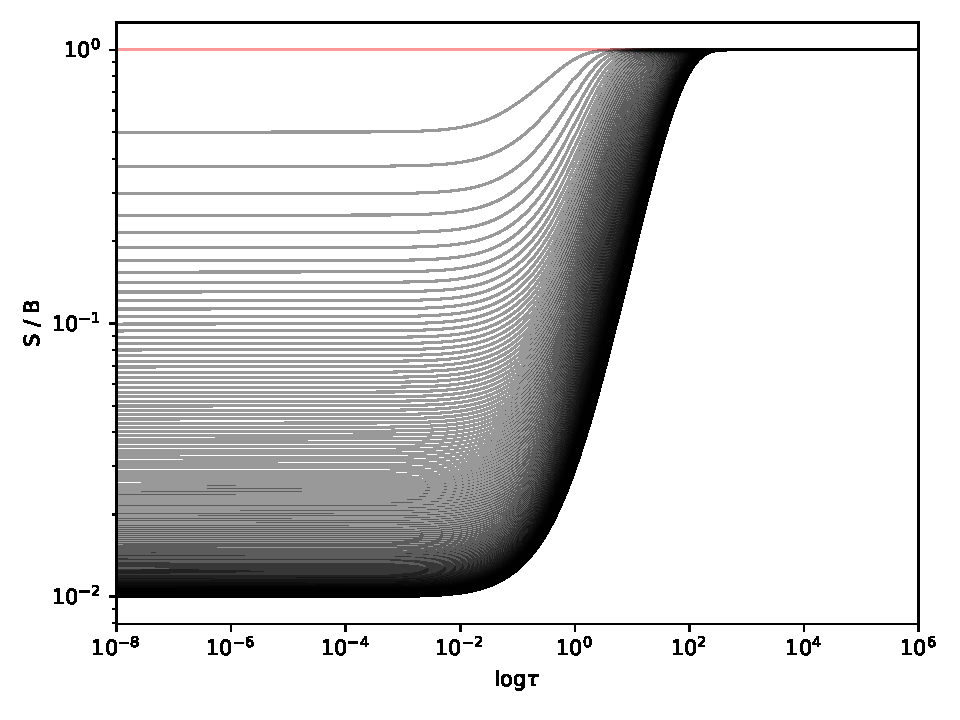
\includegraphics[width=0.75\textwidth]{S_B_convergence_noNg.pdf}
 \caption{An example convergence plot with our default parameters using ALI. Each gray line represents a new iteration, with 500 iterations total. At the surface, S/B approaches $\sqrt\epsilon$ while at depth, S/B approaches 1.}
\end{figure}

As a sanity check, we plot a spectrum generated from our model to ensure we obtain a blackbody curve. Figure 2 shows this spectrum from 3000 to 7000 $\AA$. We have attempted including an absorption line at 6564 $\AA$ (H$\alpha$). However, this feature does not show the expected Gaussian shape an absorption feature should have. This is most likely due to our Planck function being independent of $\tau$ and our temperature profile being isothermal. 

\begin{figure}[ht]
 \centering
 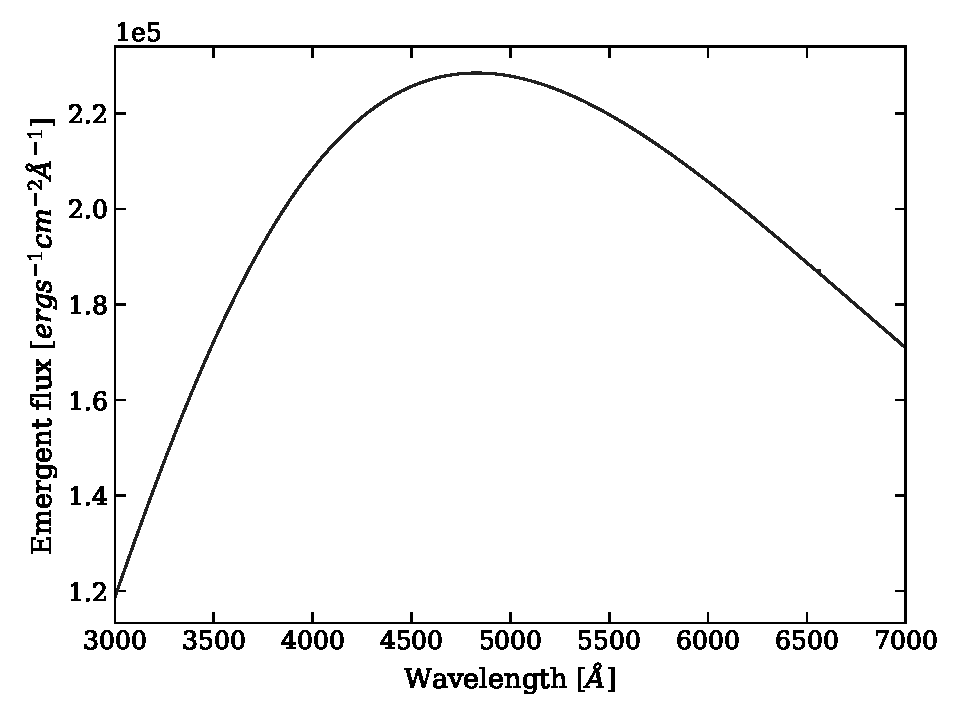
\includegraphics[width=0.75\textwidth]{test_spectrum.pdf}
 \caption{Output spectrum using the default parameters. The line feature at 6564 $\AA$ appears, however the shape is incorrect.}
\end{figure}

We test the effects of varying $\epsilon$ on the number of iterations needed to achieve convergence. Figure 3 displays these results, with each panel showing a different $\epsilon$. For $\epsilon = 1$, we have pure LTE, so S = B and S/B = 1 everywhere, so only 1 iteration is required. As $\epsilon$ approaches 0 and we deviate away from LTE, more iterations are required to achieve convergence. 

\begin{figure}[ht]
 \centering
 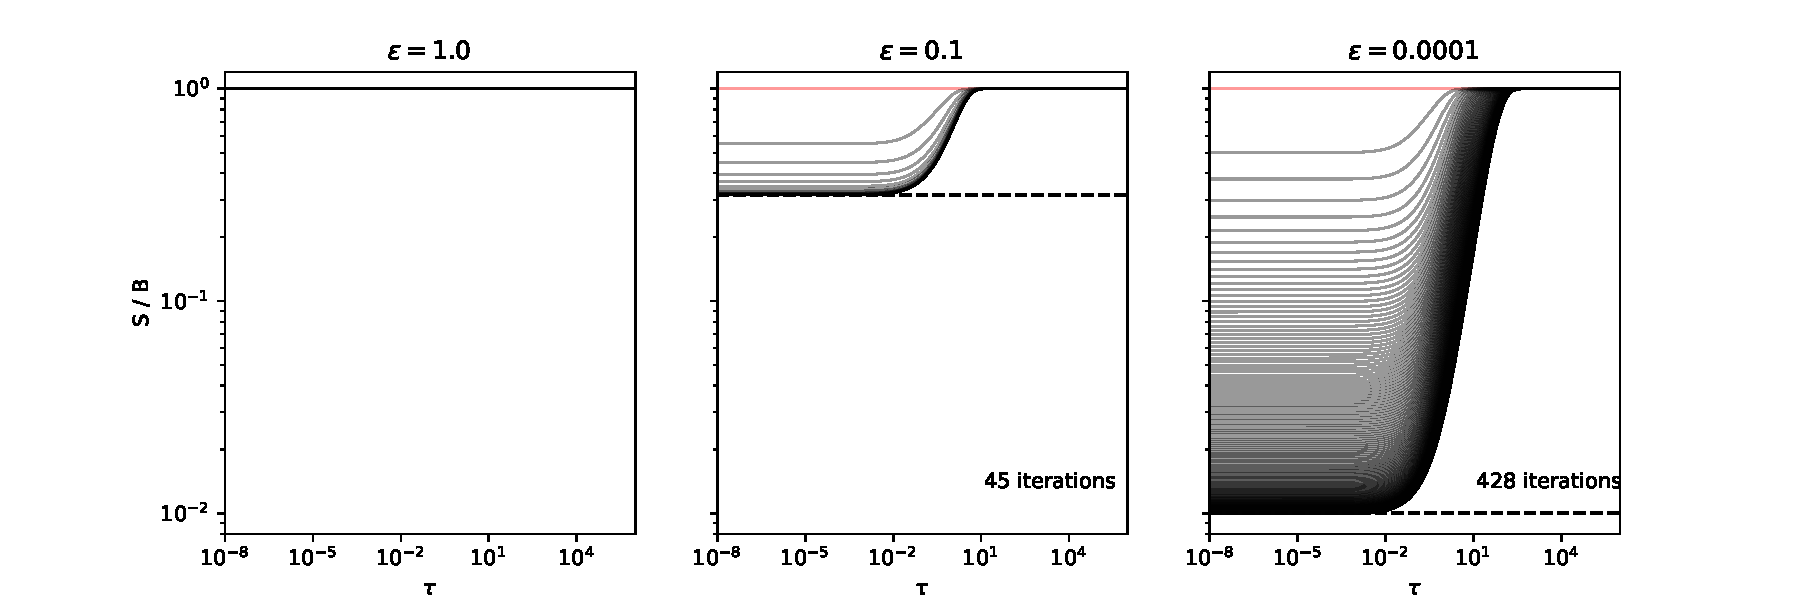
\includegraphics[width=0.99\textwidth]{eps_convergence.pdf}
 \caption{Convergence plots for different values of $\epsilon$. As $\epsilon$ approaches 0, more iterations are needed to achieve convergence at the surface.}
\end{figure}

Since J is the direction-averaged intensity, comparing our J to an analytic value is important as it directly corresponds to emergent flux from the atmosphere. In Figure 4 we show the percent difference between our J and J calculated from using a linear Planck function and the Eddington approximation: 

\begin{equation}
\begin{split}
   J(\tau) = a + b\tau + \frac{(b - \sqrt{3}a)e^{-\sqrt{3\epsilon}}}{(\sqrt{3}+\sqrt{3\epsilon})}
\end{split}
\end{equation}

In our case, the Planck function is not dependent on $\tau$, so b = 0, and a is just the Planck function. 
The largest difference between our J and the analytic solution occurs from $10^{-3} < \tau < 1$. This is expected, as this region corresponds to where the majority of the flux emerges from the atmosphere. Elsewhere, the difference between the 2 is essentially 0. We vary $\epsilon$ as well but do not obtain significant changes as $\epsilon$ changes.


\begin{figure}[ht]
 \centering
 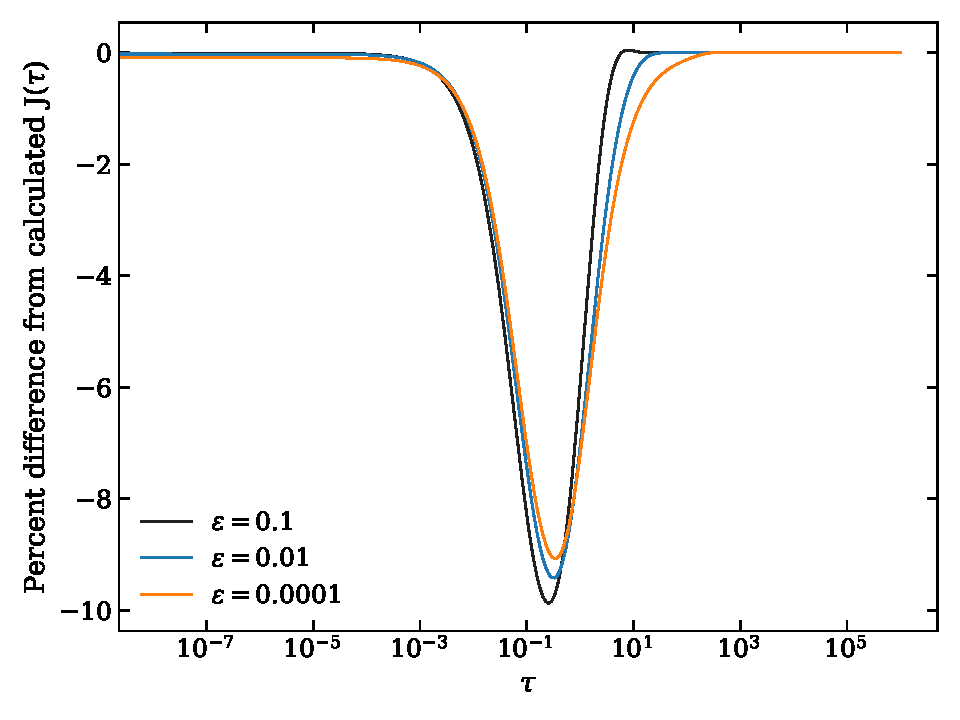
\includegraphics[width=0.75\textwidth]{J_comparison.pdf}
 \caption{Comparison of our J to the analytic solution. The greatest differences occur around $\tau = 2/3$, where we expect the greatest impact in the emergent flux from the atmosphere. Varying $\epsilon$ does not impact J to a significant degree.}
\end{figure}

We also investigate the effect of using fewer points in the Gaussian quadrature. Figure 5 shows that if we use fewer points, our calculated source function deviates significantly in the same $\tau$ regime as when we investigate J. 

\begin{figure}[ht]
 \centering
 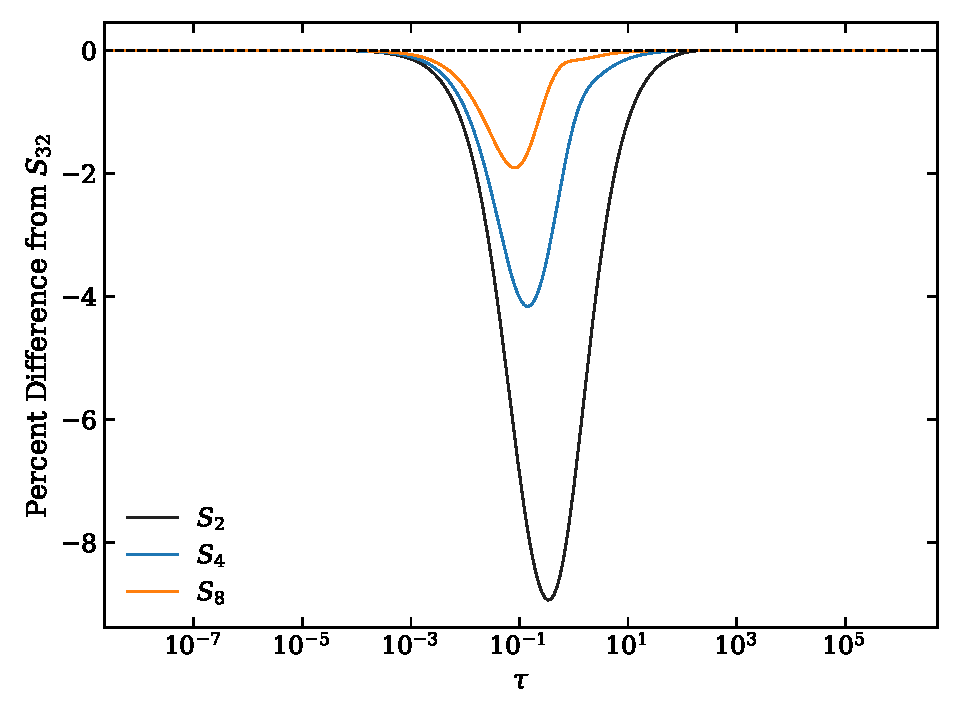
\includegraphics[width=0.75\textwidth]{quadrature.pdf}
 \caption{Deviations from 32-point Gaussian quadrature as a function of $\tau$. Similarly to Figure 4, the greatest difference occurs from $0.1 < \tau < 1$. }
\end{figure}

Finally, we investigate the effects of Ng acceleration on the speed of convergence. The left panel in Figure 6 shows the number of iterations required by each method to reach convergence at the surface for our default $\epsilon$. ALI unsurprisingly is much faster than normal LI, with Ng acceleration further improving the required amount of iterations. The right panel shows how J varies per iteration for each method. Specifically, we calculate the change in J after each iteration, normalized by the previous J, and then find the maximum change across $\tau$ at each step. This gives us an idea of how significantly J changes, with Ng acceleration obtaining smaller variations in a fewer amount of variations compared to LI and ALI. LI in particular does not do a good job of minimizing this quantity, and would require exponentially more iterations to achieve the same result.

\begin{figure}[ht]
 \centering
 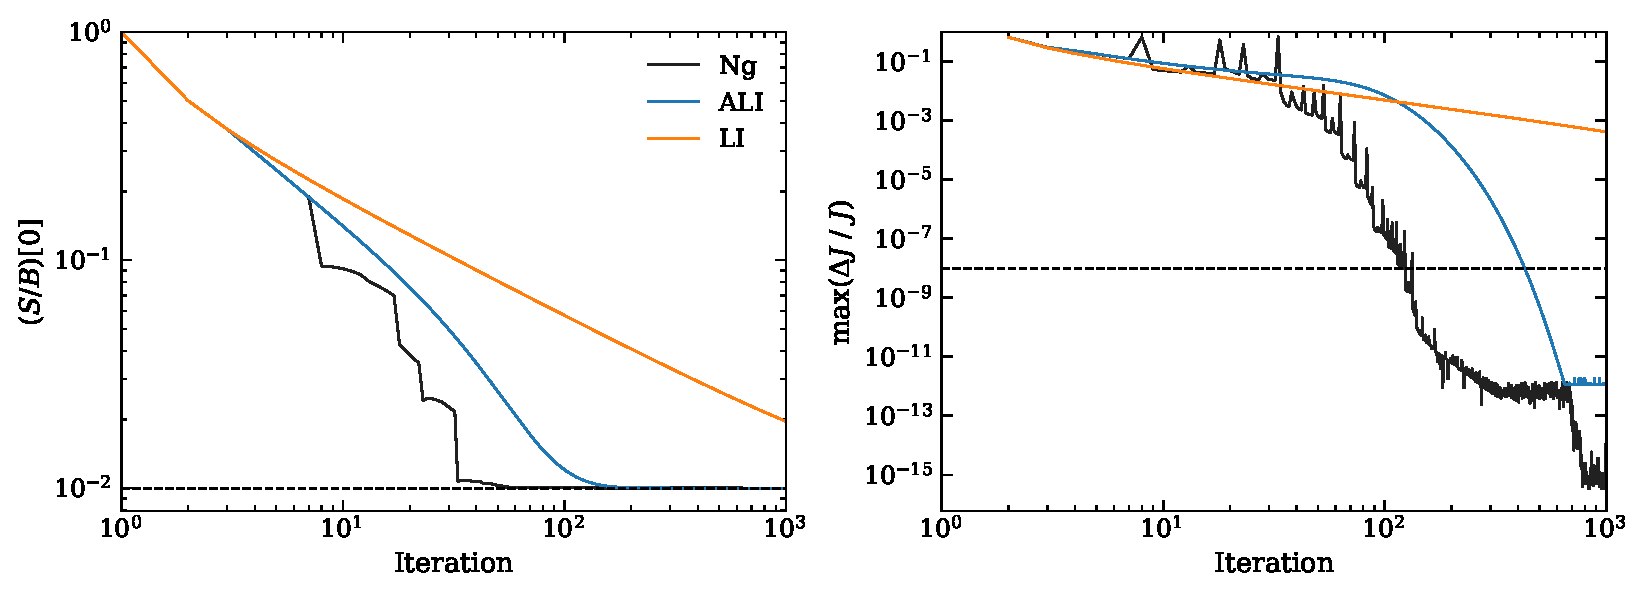
\includegraphics[width=0.99\textwidth]{iterations.pdf}
 \caption{Left: The amount of iterations required for S/B to converge at the surface for each method used in our code. Lambda iteration takes significantly longer than ALI as expected. Ng acceleration improves the required number of iterations even further. The jagged pattern is a result of how the algorithm is designed. Right: Variations in J as a function of iteration. Ng acceleration minimizes the change in J faster than ALI, though this does not take effect until about 40 iterations, and then levels off before dropping again at 700 iterations.}
\end{figure}

In Figure 7, we plot the same convergence test as Figure 1 with using Ng acceleration. It becomes clear that fewer iterations are needed, with large jumps in S/B compared to gradual steps using ALI.

\begin{figure}[ht]
 \centering
 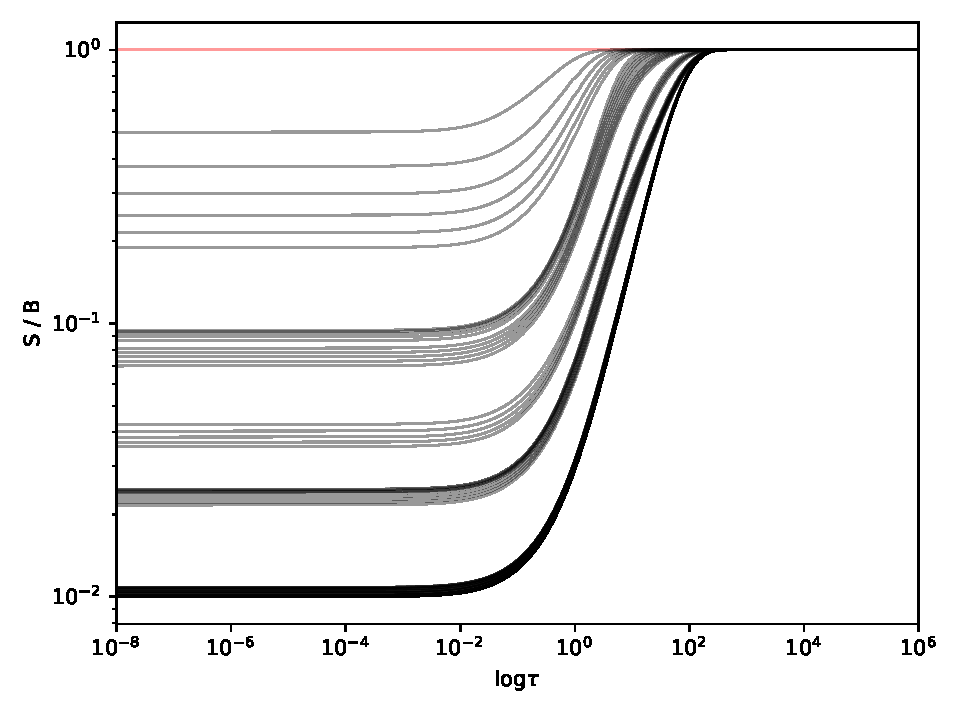
\includegraphics[width=0.75\textwidth]{doc/figs/S_B_convergence.pdf}
 \caption{The same convergence plot as Figure 1 but with Ng acceleration implemented. The number of iterations required for convergence decreases significantly.}
\end{figure}


\section{Conclusion}



\bibliography{FinalProjectReport}

\end{document}
